\usetikzlibrary{arrows.meta,calc}
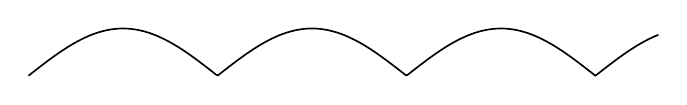
\begin{tikzpicture}[x=1cm,y=1cm,font=\normalsize,line width=.6pt]
% cusped arch line generated by absolute sine: y = 0.6*abs(sin(deg(pi*x/2.4)))
% cusps at valleys, smooth crests, matching original choice C
\draw[solid,domain=0:8,samples=400] plot (\x,{0.6*abs(sin(180*\x/2.4))});
\end{tikzpicture}
